\section{Scholarly Question Answering Framework}
\label{sec:implementation_sqa_framework}

To effectively demonstrate and evaluate the performance of the HubLink retriever within the scholarly literature search task, we developed a dedicated Python framework termed as \acrfull{sqa} system. This framework provides an environment specifically designed for the systematic testing and evaluation of diverse \gls{kgqa} approaches in academic domains. 

In the following sections, we briefly introduce each component of the \gls{sqa} system. We first introduce the key capabilities that the \gls{sqa} framework provides. Then, we outline the overall system architecture, including the different components that the framework consists of. Subsequently, each component of the framework is described in detail.

\subsubsection{Capabilities}
The \gls{sqa} framework is equipped with a range of capabilities designed to ensure flexibility, reproducibility, and comprehensive evaluation possibilities for \gls{kgqa} research. These features collectively provide a powerful toolkit for constructing, executing, and analyzing \gls{rag} pipelines tailored to scholarly information needs. Key capabilities include:

\begin{enumerate}[label=\textbf{[C\arabic*]}]
    \item \textbf{Flexible Configuration Management:} Utilizes easily modifiable JSON-based configuration files to define and serialize parameters for all system components. This ensures straightforward reproducibility and systematic modification of experiments.

    \item \textbf{Experiment Execution and Evaluation:} Automates the process of conducting experiments using pipelines defined in configuration files. It evaluates performance using a suite of relevant metrics (e.g., retrieval recall, answer relevance, factuality), stores detailed outcomes along with reproducibility information, and facilitates results visualization through generated diagrams for easier analysis.
    
    \item \textbf{Data Ingestion:} Provides modules for loading publication data and \gls{qa} pairs from standard JSON and CSV formats, serving as the foundation for knowledge base creation and evaluation datasets.

    \item \textbf{Modular RAG Pipeline:} Implements a fully customizable \gls{rag} pipeline architecture comprising pre-retrieval, retrieval, post-retrieval, and generation stages. This modularity allows easy interchanging, configuration, and testing of different algorithms or models at each stage of the workflow.
    
    \item \textbf{Scientific Text Extraction:} Integrates functionality to extract structured information from the text of publications by leveraging an \gls{llm}.
    
    \item \textbf{Knowledge Graph Integration:} Supports the modular construction and integration of diverse \glspl{kg} by providing a unified interface.
    
    \item \textbf{Semi-Automated KGQA Pair Generation}: Incorporates strategies such as graph clustering and subgraph extraction to assist in the generation of relevant \gls{qa} pairs directly from the underlying \glspl{kg}. 
    
    \item \textbf{Command-Line Interface (CLI)}: Offers a CLI application for managing configuration files, triggering data ingestion, executing individual experiments, and conducting interactive \gls{qa} sessions.

\end{enumerate}

\subsubsection{System Architecture}

\begin{figure}[p]
    \centering
    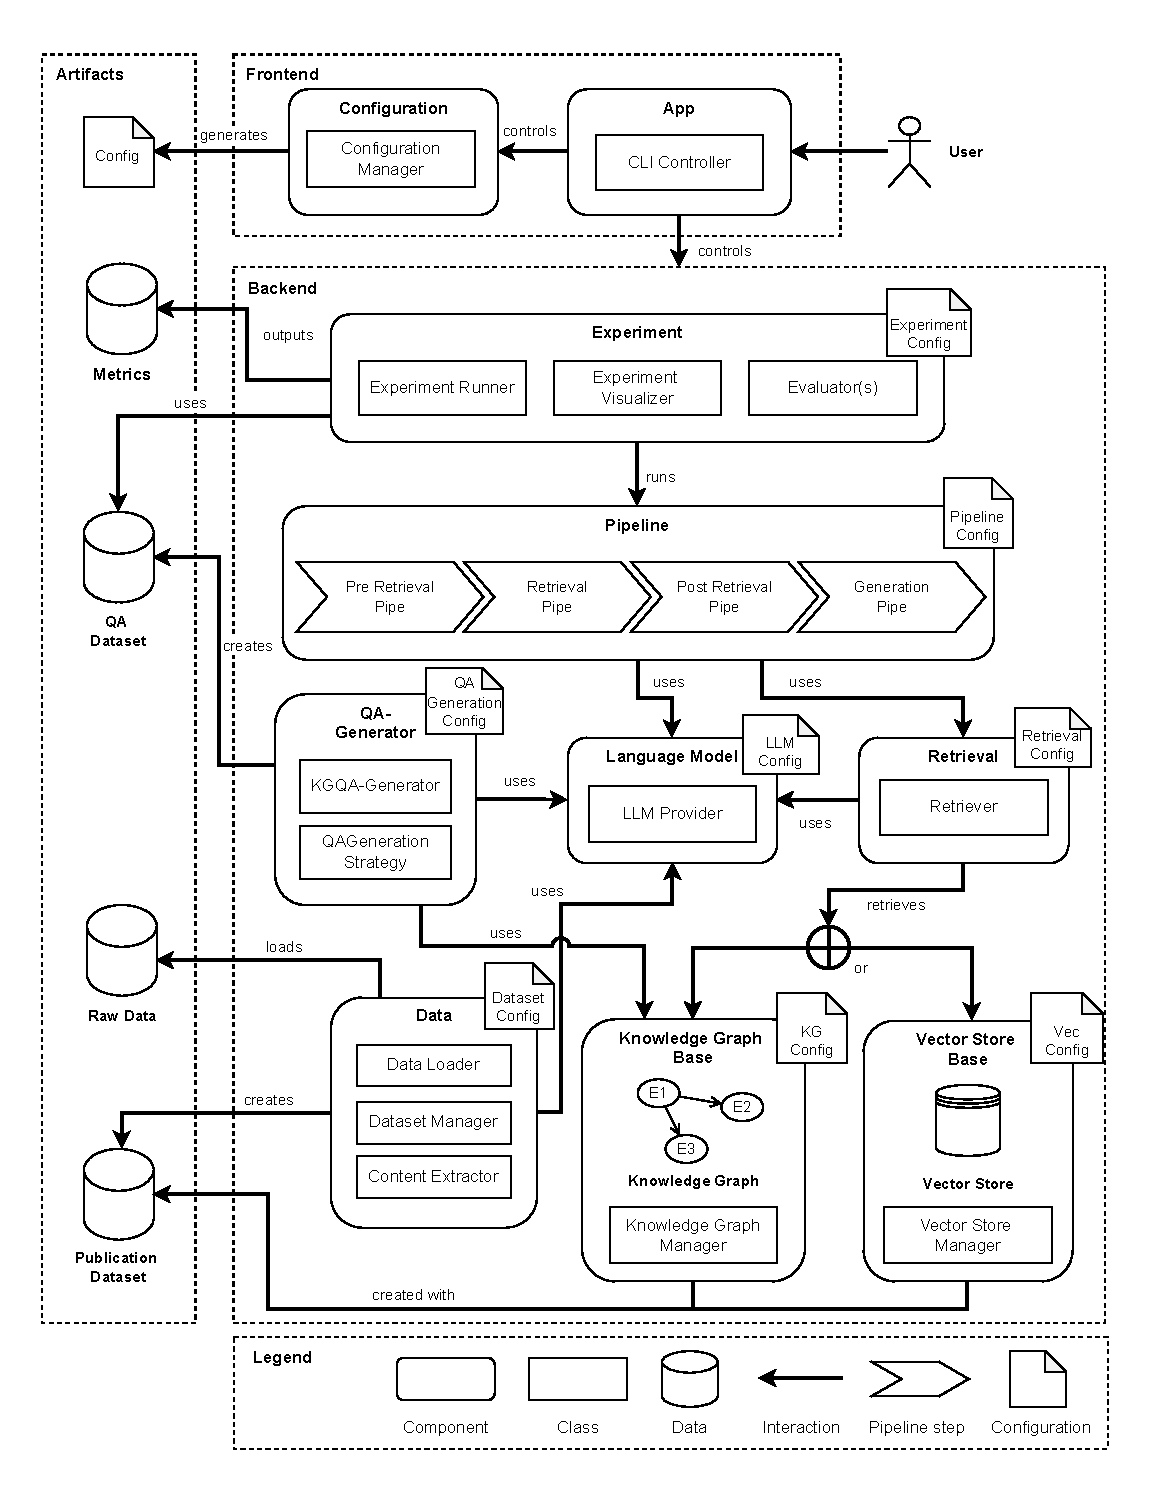
\includegraphics[width=0.99\linewidth]{figures/framework/overview-Architecture.drawio.pdf}
    \caption[SQA System Architecture]{Scholarly question-answering system architecture, illustrating key components and their primary interactions}
    \label{fig:overview_architecture}
\end{figure}

The \gls{sqa} framework is designed with extendability in mind. Consequently, it provides well-defined abstract interfaces and base classes to facilitate the straightforward integration of new \gls{kgqa} approaches, new \glspl{kg} or vector databases, different \glspl{llm}, and custom intermediate pipeline stages, ensuring the framework can adapt to future research directions and technological advancements. The framework employs a modular software architecture, as depicted in \autoref{fig:overview_architecture} to promote a clear separation of concerns, where each component encapsulates a specific set of functionalities. In the following, we briefly introduce each component of the \gls{sqa} framework before explaining them in detail:

\paragraph{Configuration Component}
The initialization and experimental setup are fundamentally based on the \emph{Configuration} component, which parses and validates JSON-based configuration files that define parameters and selected modules for all other components.

\paragraph{Data Component}
Data loading, preprocessing and distribution are the responsibility of the data component. It manages metadata and content data from publications, as well as \gls{qa} pairs from JSON and CSV sources, and makes these accessible to other parts of the system.

\paragraph{Pipeline Component}
The core logic of the question-answering process resides within the \emph{Pipeline} component. This component orchestrates the sequence of pipeline operations (pre-retrieval processing, context retrieval, post-retrieval processing, and final answer generation). 

\paragraph{Retriever Component}
Integrated closely with the pipeline, the \emph{Retriever} component performs the task of searching the designated \gls{kb} (\gls{kg} or vector index) to find contextually relevant information passages or facts relevant to the input question.

\paragraph{Language Model Component}
A unified interface for interacting with local or API-based \glspl{llm} is provided by the language model component. It handles \gls{llm} access for other components of the system and parses the response.

\paragraph{Knowledge Base}
A \gls{kb} stores and provides access to the data in the system. In the system, two types of \glspl{kb} are supported, which are \glspl{kg} and vector indices. Both are unified in the knowledge base component.

\paragraph{Experiment Component}
The experiment component provides the functionality to perform systematic evaluations. It iterates over specified configurations, executes the \gls{qa} pipeline for each test question, collects results, computes relevant \gls{rag} metrics, and stores these findings for later analysis.

\paragraph{QA Generator Component}
This component helps to create evaluation datasets by implementing semi-automated methods to generate \gls{kgqa} pairs from a \gls{kg} using an \gls{llm}.

\paragraph{App Component}
User interaction is managed through the app component, which offers a CLI application. This tool allows users to manage configurations, execute experiments, ingest data, and perform interactive querying of pipelines.

\subsection{Data Component}
\label{sec:sqas_architecture_inputs_outputs}

The \gls{sqa} system processes several types of data and features the structured \gls{llm}-based extraction of text. This section details the primary inputs and outputs handled by the system and describes the process of extracting structured data from paper texts.

\subsubsection{Inputs}

\begin{figure}[t]
    \centering
    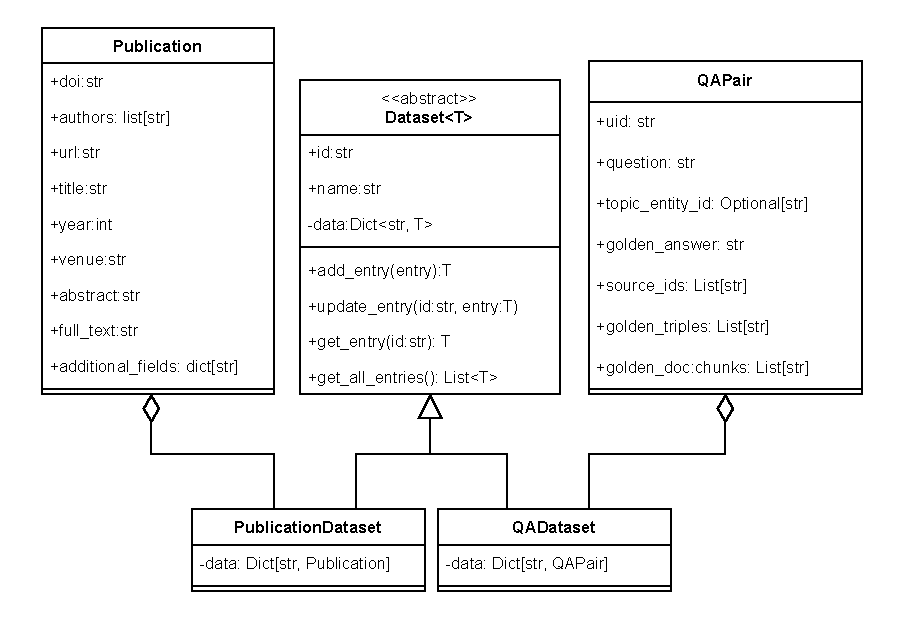
\includegraphics[width=0.99\linewidth]{figures/framework/figures-Input_data_models.drawio.pdf}
    \caption[Input Data Models of the SQA System]{Input data models of the \gls{sqa} system.}
    \label{fig:input_data_models}
\end{figure}

Any data that is inserted into the system has to be converted to either a \texttt{Publication} or \texttt{QAPair} object as depicted in \autoref{fig:input_data_models}. We introduce them in the following:

\paragraph{Publication Data:} 
An important data input of the \gls{sqa} framework is the metadata and content texts of scientific publications. These are ingested into the system from raw data, for example, in JSON format. For our experiments, we implemented a dedicated \texttt{JsonDataLoader}, which loads the publication data and converts it into the internal \texttt{Publication} data model that encapsulates both metadata and available full text for each scientific publication. To handle multiple publications, the \texttt{PublicationDataset} data model is used. This data model stores a collection of publications and provides easy access to them. The dataset is managed by the \texttt{DatasetManager} class, which enables other components to access datasets by providing configuration files. The manager then initiates the loading and handles the persistence.

\paragraph{Question-Answer Pair Data:} 
Question-answer pairs include the questions and ground truth to conduct the experiments. These are internally stored as \texttt{QAPair} objects in the \gls{sqa} system and loaded from data loader implementations from raw formats such as CSV. For our experiments, we implemented a \texttt{CSVDataLoader} that allows the serialized \gls{kgqa} dataset to be imported and used for the experiments. The \texttt{QAPair} data model has the following attributes:

\begin{enumerate}
    \item \textbf{UID:} A unique identification identifier that uniquely identifies the specific question-answer pair.
    \item \textbf{Question:} The natural language question posed to the \gls{qa} system.
    \item \textbf{Topic Entity:} An optional field specifying an entity within the target \gls{kg}, which potentially serves as an entry point for certain retrieval algorithms. It is optional as not all retrievers require this information.
    \item \textbf{Golden Answer:} A reference answer to the question, formulated in natural language, considered correct for evaluation purposes.
    \item \textbf{Golden Triples:} A set of triples present in the target \gls{kg} that represent the factual basis for the \emph{Golden Answer}.
    \item \textbf{Golden Text Chunks:} The text passages from source publications containing information that correspond to the \emph{Golden Answer} and align with the \emph{Golden Triples}.
    \item \textbf{Source IDs:} Identifiers of the source publications from which the \emph{Golden Answer}, \emph{Golden Triples}, and \emph{Golden Text Chunks} were derived.
\end{enumerate}

Similarly to the publication data, a collection of \texttt{QAPair} is handled by a \texttt{QADataset} data model. This model handles the access to the pairs and their persistence.


\subsubsection{Outputs}
Depending on the executed workflow (e.g., experimentation, interactive querying, \gls{qa} generation), the \gls{sqa} system produces several outputs:

\paragraph{Experiment Results:} 
When running an experiment, for each question several outputs are produced. These outputs include the generated answer and the retrieved context that both relate to the provided question. These outputs are then evaluated against the golden ground truth data provided by the \texttt{QADataset} using dedicated \texttt{Evaluator} objects. These produce comprehensive evaluation reports containing various \gls{rag} metrics (e.g., context relevance, answer faithfulness) and other measurements, which are then aggregated and exported in \texttt{CSV} format. Subsequently, an \texttt{ExperimentVisualizer} can be used to generate plots and tables to visualize the results.

\paragraph{Simple Answer:}
When executing a \gls{rag} pipeline in interactive mode, the primary output returned to the user is the generated natural language answer to the question posed.

\paragraph{QA Generation Data:} 
Another output comprises the semi-automatically generated \texttt{QAPair} objects, which are stored in a \texttt{QADataset} structure and serialized into \texttt{CSV} format for subsequent use in evaluations.

\subsubsection{Data Extraction}
The \gls{sqa} system also provides the ability to extract scientific content directly from the text of scientific publications. This process, orchestrated by the \texttt{ContentExtractor} class using a configured \gls{llm}, transforms unstructured text into structured data suitable for enriching \glspl{kg}. The extraction process involves the following steps:

\begin{enumerate}
    \item \textbf{Text Chunking:} The source text of the publication is segmented into smaller, manageable chunks suitable for processing by the context window limits of the \gls{llm}.
    \item \textbf{Chunk Extraction:} Each text chunk is processed by the \gls{llm}. To enhance completeness, this extraction is done multiple times for the same chunk. In subsequent extractions for the same chunk, previously extracted information is aggregated and provided back to the \gls{llm} as context to minimize redundancy.
    \item \textbf{Tracing:} Each extracted data item is mapped back to its location in the original publication source. This trace provides provenance for the information extracted.
\end{enumerate}

As mentioned above, the core extraction mechanism involves prompting the \gls{llm}. This is accomplished by populating a predefined \texttt{JSON} schema which defines the target information types, attributes, and relationships to be extracted (e.g., research methods used, research questions, key findings). The task of the \gls{llm} is to analyze the provided text chunk and accurately populate this schema with corresponding information found within the text. The data extracted from the schema can subsequently be utilized, for instance, in the construction of a \gls{kg}.

\subsection{Configuration Component}
\label{sec:sqas_architecture_configuration}

A primary goal during the development of the \gls{sqa} system was to ensure the easy definition and reproducibility of experiments. To achieve this, the system utilizes configuration files stored in \texttt{JSON} format. This storage method serializes configurations, enabling their persistence for future use and allowing experiments to be repeated accurately by using the corresponding files.

\begin{figure}
    \centering
    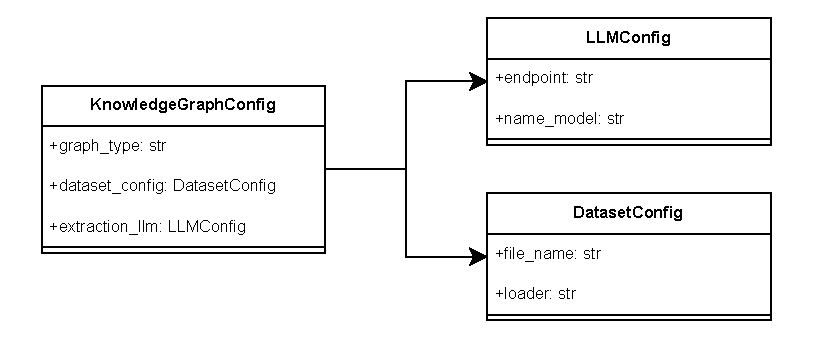
\includegraphics[width=0.90\linewidth]{figures/framework/figures-Bsp_Config_Model.drawio.pdf}
    \caption[Knowledge Graph Configuration Model]{The configuration model for a Knowledge Graph in the SQA system.}
    \label{fig:config_model}
\end{figure}

Each component of the \gls{sqa} system is controlled through a dedicated configuration file that defines its required parameters. An important characteristic of a configuration is that it can be hierarchically defined, meaning that one configuration may include another. \autoref{fig:config_model} shows the \gls{kg} configuration model as an example. It illustrates the parameters required, demonstrating that configurations can contain both primitive data types, such as strings and integers, and complex structures, like nested configuration objects.

To load the JSON files into the \gls{sqa} system the \texttt{ConfigurationManager} is responsible. This manager interprets the file to confirm that it is correctly structured and provides the filled configuration object to the relevant component that needs to be initialized. Furthermore, for reproducibility and caching, it is essential to determine whether two configurations are identical. This is achieved by calculating a cryptographic hash value for each configuration object. By calculating this hash over the content of the configuration, we ensure that the values of two configurations are only identical if and only if their contents are identical. This mechanism makes it easy to determine whether two configurations are the same. This functionality is used by components in the system to avoid duplicate instantiation in caching scenarios such as storing \gls{llm} models or \glspl{kg}. 



\subsection{Pipeline and Pipes Component}

The \gls{rag} process is implemented within the \gls{sqa} system using a pipeline architecture facilitated by the LangChain library\footnote{\url{https://www.langchain.com/} [last accessed on 12.05.2025]}. This pipeline accepts a question and, optionally, a topic entity as input. The pipeline processes this input and returns a \texttt{PipeIO} object populated with the results. The \texttt{PipeIO} object acts as a data container, progressively accumulating information such as the retrieved contexts and the generated answer as it traverses the pipeline stages. It also collects tracking data like carbon emissions or \gls{llm} token usage. 

In the following sections, we first describe the retrieval pipeline. Then, we detail the \texttt{PipeIO} data model.

\subsubsection{Retrieval Pipeline}
A standard pipeline comprises four distinct stages, referred to as \emph{pipes}. These pipes are executed sequentially in a predefined order: Execution starts with the \emph{Pre-Retrieval Pipe}, followed by the \emph{Retrieval Pipe}, then the \emph{Post-Retrieval Pipe}, and concludes with the \emph{Generation Pipe}. These pipes are explained in the following:


\paragraph{Pre-Retrieval Pipe:} 
This pipe is responsible for processing the input question before retrieval takes place. For example, the question given as input into the pipeline can be expanded to include synonyms or related terms to improve recall.

\paragraph{Retrieval Pipe:}
This is the pipe that is responsible for the extraction of relevant contexts from the underlying \gls{kb}. All retrievers are applied within this pipeline step. The task of the retriever is to identify and retrieve relevant context passages or structured data from the designated \gls{kb}. The retrieved contexts are then stored in the \texttt{PipeIO} object. In addition, certain retrievers may generate a final answer directly. If the retriever does not generate an answer, a subsequent \emph{Generation Pipe} is required to generate the answer.

\paragraph{Post-Retrieval Pipe:} 
This optional stage processes the contexts retrieved in the previous stage. Common operations include filtering irrelevant passages, reranking of contexts based on relevance or other criteria, or selecting a subset of contexts based on a specified criteria.

\paragraph{Generation Pipe:}
This pipe is responsible for synthesizing the final natural language answer. A configured \gls{llm} is invoked, provided with the original question and the retrieved contexts. The task of the \gls{llm} is to generate a coherent and factually grounded answer based on this input. The generated answer is then stored in the \texttt{PipeIO} object, completing the pipeline execution. This stage is optional if the retriever already produced a final answer.


\subsubsection{PipeIO Datamodel}
\begin{figure}[t]
    \centering
    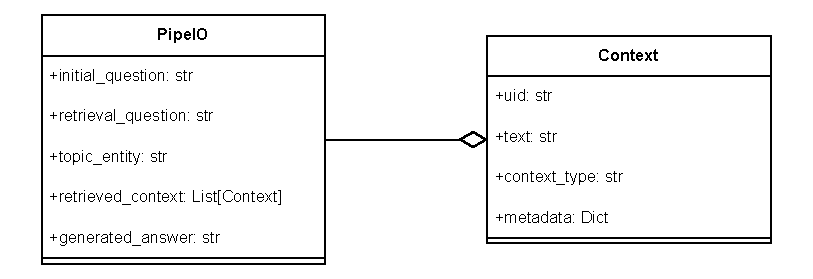
\includegraphics[width=0.90\linewidth]{figures/framework/figures-pipeIO_model.drawio.pdf}
    \caption[UML Diagram for the PipeIO Data Model in the SQA Framework]{The UML Diagram of the PipeIO model.}
    \label{fig:pipeio_model}
\end{figure}

The data model of the \texttt{PipeIO} object is shown in \autoref{fig:pipeio_model}. It contains several attributes that are populated by the individual pipes in the pipeline. Initially, the \texttt{PipeIO} data model is created by the pipeline, where the attributes \texttt{initial\_question}, \texttt{retrieval\_question}, and \texttt{topic\_entity} are initialized. The distinction between these two types of question exists because when the question is modified by the pre-retrieval pipe, the original question should still be saved. Consequently, the \texttt{initial\_question} attribute is \texttt{read-only}, while \texttt{retrieval\_question} can be modified. Furthermore, the topic entity can optionally be added. This allows retrievers to have an entry point in the \gls{kg} if they require it. Moreover, the \texttt{PipeIO} object contains the attributes \texttt{retrieved\_context} and \texttt{generated\_answer}. These attributes are filled during execution. 



\subsection{Retriever Component}
\label{sec:sqas_architecture_retriever}

\begin{figure}[t]
    \centering
    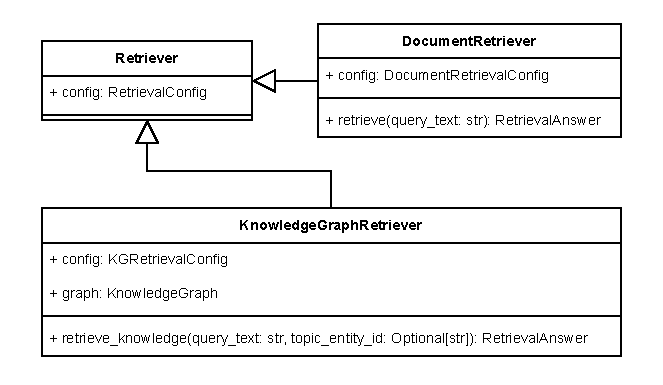
\includegraphics[width=0.80\linewidth]{figures/framework/figures-Retriever_UML.drawio.pdf}
    \caption[UML Diagram for Retrievers in the SQA Framework]{The UML diagram for retrievers in the SQA framework.}
    \label{fig:retriever_model}
\end{figure}

The main class in the retrieval component is the \texttt{Retriever}, which is responsible for finding relevant contexts from a \gls{kb} to answer a question. There are two sub-classes available for the \texttt{Retriever}: the \texttt{DocumentRetriever} and the \texttt{KnowledgeGraphRetriever}, each handling different types of data:

\paragraph{Document-based Retriever} works with text documents as input sources, specifically the full text of scientific publications. Unlike the \gls{kg} variant, the \texttt{DocumentRetriever} is not bound to a specific \gls{kb}. Instead, the corresponding \texttt{DocumentRetrievalConfig} specifies the configuration of the dataset, which contains the data that should be used for retrieval instead of a \gls{kg}.

\paragraph{Knowledge Graph-based Retriever} operates directly on a \gls{kg}. Instead of documents, it uses a \gls{kg} as the underlying data store. The configuration for the \gls{kg} is provided with the \texttt{KGRetrievalConfig} during the initialization of the retriever.

Once the retriever is implemented in the system, it is used in a pipeline to allow the retrieval of context for questions and to generate answers.

\subsection{Language Model Component}
\label{sec:sqas_architecture_language_model}

\begin{figure}[t]
    \centering
    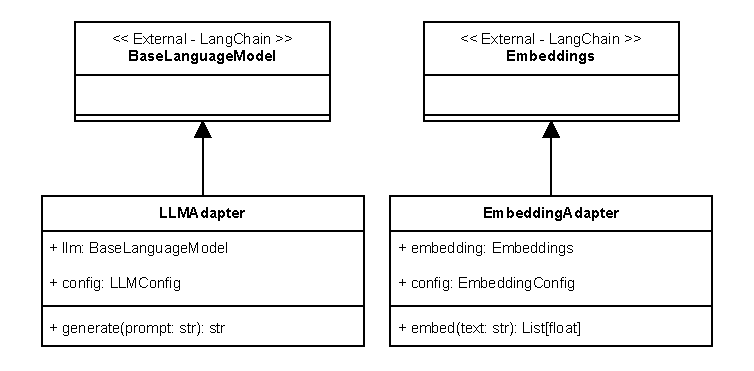
\includegraphics[width=0.80\linewidth]{figures/framework/figures-llm_model.drawio.pdf}
        \caption[UML Diagram for LLM and Embedding Adapters]{The UML diagram for the LLM adapter and Embedding adapter classes of the SQA system.}
        \label{fig:llm_model}
    \end{figure}

Since many components of the \gls{sqa} system work with \glspl{llm}, a dedicated \emph{Language Model} component is provided. This component offers a unified interface to make requests to an \gls{llm}. The requests, in conjunction with their corresponding configuration, are handled by the \texttt{LLMProvider}, which is responsible for initializing the model and establishing the connection.

The implementation of the models is achieved through the adaptation of the \texttt{BaseLanguageModel} and \texttt{Embeddings} classes from the LangChain\footnote{\url{https://python.langchain.com/docs/integrations/chat/} [last accessed on 28.01.2025]} library. The advantage of using the LangChain framework lies in its support for a wide range of models, a well-maintained interface, and easy integration of new models. Two types of adapters are implemented, which are shown in \autoref{fig:llm_model}. The \texttt{LLMAdapter} is responsible for sending requests to the \gls{llm} and processing the responses. The \texttt{EmbeddingAdapter}, on the other hand, handles the transformation of texts into vectors.

\subsection{Knowledge Bases Component}
\label{sec:sqas_architecture_knowledge_bases}

\begin{figure}[t]
    \centering
    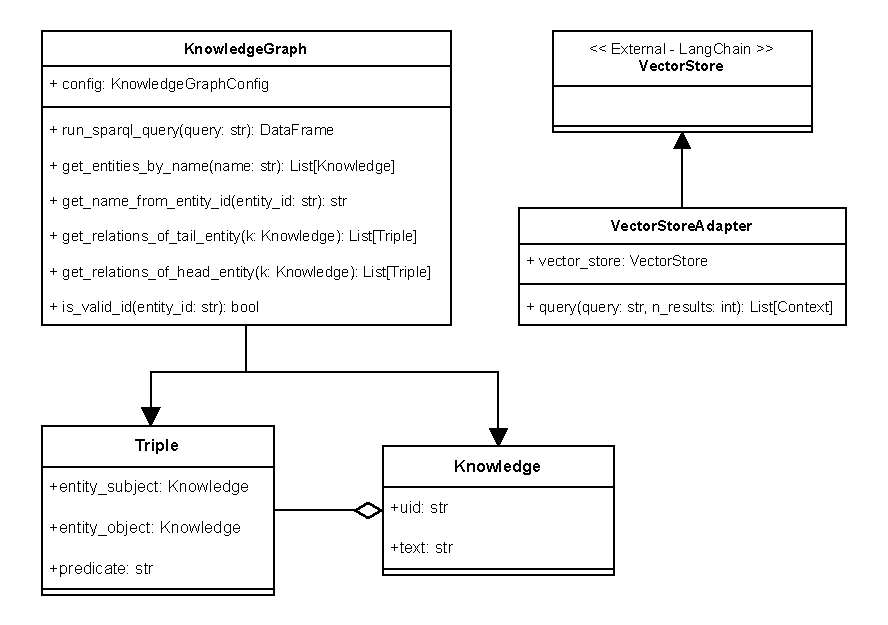
\includegraphics[width=0.99\linewidth]{figures/framework/figures-Knowledge_bases_uml.drawio.pdf}
    \caption[UML Diagram for KGs and Vector Stores]{The UML diagram for the knowledge graph and vector store.}
    \label{fig:knowledge_bases_model}
\end{figure}

The \gls{sqa} system provides two different types of \glspl{kb} as shown in \autoref{fig:knowledge_bases_model}: \glspl{kg} and vector stores. These \glspl{kb} can be used by retrievers to find relevant contexts for answering questions. In the following, we detail their implementations in the \gls{sqa} system:

\paragraph{Knowledge Graphs} are represented as \gls{rdf} graphs in the \gls{sqa} system. These graphs consist of triples represented with the \texttt{Triple} data model, which consists of \texttt{Knowledge} objects as shown in \autoref{fig:knowledge_bases_model}. Moreover, to manage and provide \texttt{KnowledgeGraph} objects in the \gls{sqa} system, the \texttt{KnowledgeGraphManager} is responsible. This manager initializes the graphs based on the provided configuration and caches their connection to allow other components to query the graph. The preparation or creation of a \gls{kg} is facilitated by the \texttt{KnowledgeGraphFactory}. This factory receives the graph configuration file and initializes or creates the \gls{kg} based on the given parameters.

\paragraph{Vector Stores} are specialized data structures that enable efficient vector storage and querying. They are used to store texts that have been transformed into a low-dimensional vector space using an embedding model. These vectors can then be used to calculate the similarities between texts. In the \gls{sqa} system, the \texttt{VectorStore} implementation from the LangChain library is adapted using a \texttt{VectorStoreAdapter}. Similarly to knowledge graphs, a \texttt{VectorStoreManager} is responsible for initializing, managing, and providing the vector stores.

\subsection{Experiment Component}

\begin{figure}[t]
    \centering
    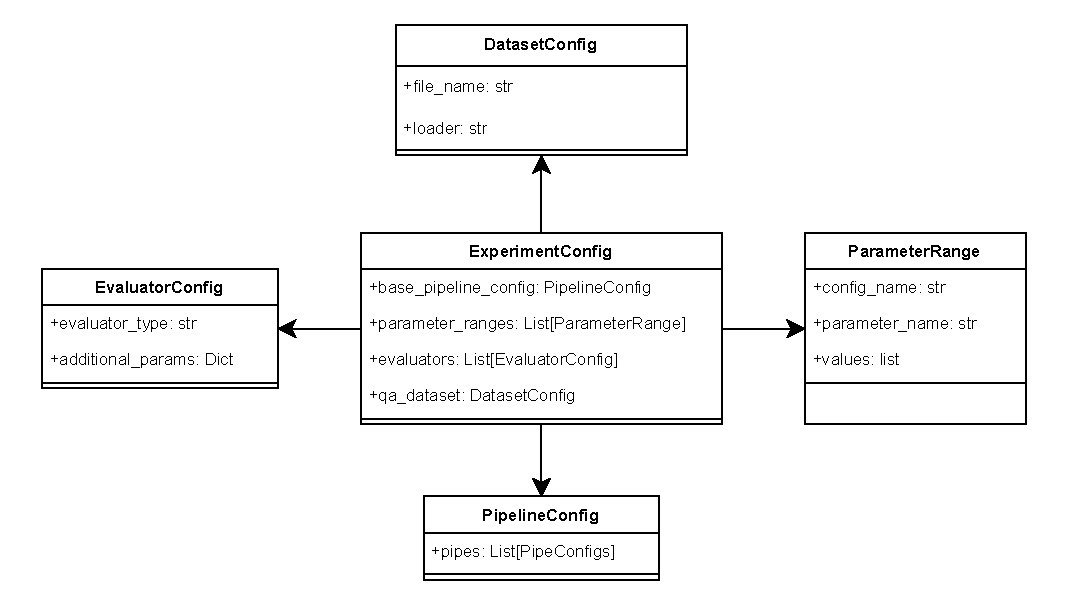
\includegraphics[width=0.99\linewidth]{figures/framework/figures-Experiment_model.drawio.pdf}
    \caption[UML Diagram for a Experiment Configuration]{The UML diagram for the experiment configuration}
    \label{fig:experiment_model}
\end{figure}

One of the main features of the \gls{sqa} system is the execution of experiments. These are defined using configuration files as described in Section~\ref{sec:sqas_architecture_configuration}. The UML diagram of an \texttt{ExperimentConfig} is shown in \autoref{fig:experiment_model}. This configuration contains all parameters necessary for conducting an experiment:

\begin{itemize}
    \item \textbf{Base Pipeline Config} is the configuration of the pipeline used for answering questions. It contains all the necessary parameters to initialize an \gls{rag} pipeline.
    \item \textbf{Parameter Ranges} are a list of parameters that allow varying the pipeline parameters within an experiment, which is useful for studying the effects of parameters on the results. The parameter configurations specified here are used by the \texttt{ExperimentRunner} to create multiple pipelines based on the base pipeline configuration, which are then executed in batch.
    \item \textbf{Evaluators} is a list of configurations for evaluators. These are classes in the \gls{sqa} system responsible for creating \gls{rag} metrics for the experiment.
    \item \textbf{QA Dataset} is the configuration of the \texttt{QADataset} used for the experiment. This contains the questions to be answered in the experiment, along with the corresponding ground truth data for evaluation.
\end{itemize}

The \texttt{ExperimentRunner} class is responsible for executing the experiment based on a configuration. This class takes the configuration and prepares the pipelines, which are then executed sequentially to fill the \texttt{PipeIO} object with data. Subsequently, the results of the pipeline are evaluated using the evaluators, which are also prepared by the runner. After the experiment has been conducted, the \texttt{ExperimentVisualizer} class is responsible for visualizing the results in diagrams and tables.

\subsection{Question Answering Generator Component}
\label{sec:qa_generator}
This component is responsible for the semi-automated creation of \gls{kgqa} pairs, which are stored internally as \texttt{QAPair} data models. The \gls{sqa} framework implements two different strategies for generating these \texttt{QAPair} objects: the \emph{Clustering Strategy} and the \emph{Subgraph Strategy}.

In the following, we first describe the clustering and subgraph strategy. Then, we explain the context and answer validation of the generated questions and answers.

\subsubsection{Clustering Strategy}
A significant challenge in generating \gls{kgqa} datasets is ensuring the completeness of the ground truth, particularly when an answer corresponds to multiple triples in the graph \cite{steinmetz_what_2021}. Ideally, the ground truth associated with a question should encompass all valid, relevant triples from the \gls{kg}. Incomplete ground truth can lead to misleading evaluations where systems are penalized for retrieving valid facts not included in the reference set. The \emph{Clustering Strategy} aims to address this challenge by identifying and grouping all potentially relevant facts before generating the question. The strategy operates as follows:

\begin{enumerate}
    \item \textbf{Provide Parameters:} The strategy is initialized with various parameters. One essential parameter is the topic entity from the graph. This entity serves as the starting point for the triple collection and is stored as the topic entity in the resulting \texttt{QAPair} object.
    
    \item \textbf{Build Publication Subgraphs:} The first step is to collect the subgraph for each publication containing triples that conform to user-provided restrictions. This requires the \emph{predicate type restriction} parameter, specifying the predicate identifier used to initially select relevant subgraphs. For each matching triple containing this predicate, the graph is traversed backward to locate the unique \enquote{paper type} triple that acts as the root node for the subgraph of the publication. Once the root is found, the strategy builds the subgraph by traversing outgoing edges until leaf nodes are reached. The result is a collection of publication subgraphs, each guaranteed to contain the specified predicate type.
    
    \item \textbf{Extract Values:} In the second step, the strategy extracts values of interest from each publication subgraph found previously, using a \emph{predicate value restriction} parameter defining the target predicate names. The strategy searches each subgraph for triples with matching predicates. Starting from these matching triples, it traverses all outgoing paths to leaf nodes, extracting their values. This produces a mapping from each extracted value of interest back to its source publication subgraph.
    
    \item \textbf{Cluster Values:} These extracted values of interest are then embedded into a vector space using a selected embedding model and subsequently clustered using the DBSCAN \cite{ester_density-based_1996} algorithm. This step forms clusters grouping semantically similar values. The mapping back to the source publication for each value is maintained throughout this process.
    
    \item \textbf{Additional Restrictions:} Based on these semantically coherent clusters, additional restrictions, which are also provided as parameters, can be applied. Each cluster is processed, and relevant triples conforming to these new restrictions are extracted from the associated publication subgraphs and added to the data payload of the cluster. The result is a set of clusters, each representing a semantic group of values and enriched with additional context triples.
    
    \item \textbf{LLM-based Generation:} After the clustering is done, the next step is the generation of the question and answer. Here, a \emph{template text} and \emph{additional instructions} for the \gls{llm} are provided as parameters to the strategy. The template is a question with placeholders to guide the \gls{llm} in the generation process, and the additional instructions are appended to the base prompt to further fine-tune the generation process. To generate the question and answer, the clusters are processed one by one and forwarded to the \gls{llm} with the prepared prompt. The \gls{llm} then generates a question and a corresponding answer given the data from the cluster, the template and instructions.
    
    \item \textbf{Prepare Ground Truth:} The triples accumulated within each cluster during the preceding steps serve as the ground truth. These are stored alongside the generated question and answer in the \texttt{QAPair} object.
    
    \item \textbf{Manual Validation:} Due to the potential for \gls{llm} hallucination or failure to adhere to instructions or templates, a final manual validation step is essential. The generated question and answer are checked for correctness, coherence, and adherence to the template. Consequently, the relevance and correctness of the collected ground truth triples must be manually verified.
    
\end{enumerate}

In the following, we illustrate an example to clarify the functionality of the clustering strategy. For this purpose, we use the following question template: \enquote{Which publications investigate the research object [research object name] and evaluate the sub-property [sub-property name]?}.

First, we need to ensure that all subgraphs containing the required information are fetched for further processing. In the case of the \gls{orkg}, we can directly use the unique identifier of the \emph{Research Object} predicate: $P162024$. This ensures that all publications that contain research objects are considered by the strategy.

Next, we define the list of predicate names that should be clustered from the subgraphs. Based on the question, we must specify the corresponding predicate names under which the requested information is stored in the graph. In our case, the predicates are labeled as \texttt{Research Object} and \texttt{Sub-Property}. In addition, further parameters can be defined to influence how the information is added to the clusters. For example, we can decide to split the clusters. In this case, the retrieved values are not added to the current cluster. Instead, a separate copy of the cluster is created for each value. This is desired for our question, as we do not want to collect all possible values of research objects and sub-properties in a single cluster but rather focus on specific instances.

At this step, each cluster contains all the publications of the dataset that investigate the same research object and evaluate the same sub-property. These clusters are now individually forwarded to the \gls{llm} that generates the question and the answer based on the triples in the cluster.

% This strategy allows for the creation of complex question-answer pairs. A major advantage over approaches solely reliant on SPARQL templates is the ability to group related information based on semantic similarity via clustering, rather than relying solely on explicit graph patterns. Furthermore, users provide predicate identifiers or names rather than formulating potentially complex SPARQL queries. Consequently, the strategy allows to automate the extraction and preparation of relevant graph data for generation.

\subsubsection{Subgraph Strategy} 
The second available strategy is the \emph{Subgraph Strategy}, which generates diverse question-answer pairs related to a single publication at a time. Unlike the cluster-based approach, this strategy does not inherently generate questions spanning multiple publications. Furthermore, it is less restrictive, which can enable the generation of a wider variety of question types. The strategy operates as follows:


\begin{enumerate}
    \item \textbf{Input Definition:} The strategy requires a publication entity from the \gls{kg} as input, which acts as a \emph{topic entity} identifier.

    \item \textbf{Subgraph Extraction:} Starting from the publication entity, the graph is traversed to extract the subgraph of the publication by traversing the graph until the leaf nodes are reached. However, this subgraph is limited to a predefined size to fit within the context window of the \gls{llm}.

    \item \textbf{LLM-based Generation:} This subgraph is then provided to the \gls{llm} with the instruction to generate both a relevant question and the corresponding golden answer. The generation process is guided by requiring the \gls{llm} to output a \texttt{JSON} structure containing the generated question, the answer and the specific subgraph triples that were used as the basis for generation.
\end{enumerate}


% \subsubsection{Techniques for Quality Assurance}
% To ensure the quality of the created \gls{qa} pairs, various techniques are employed, which are described below:

% \paragraph{Triple Tracing:} The \gls{sqa} system allows to extract structural data from the texts of publications. During this extraction, a tracing is generated and stored to map each generated triple back to the original text. This allows transparency and helps solve a challenge. Since the \gls{sqa} system also supports retrievers that work with documents (see Section~\ref{sec:sqas_architecture_retriever}), it is important to provide not only the golden triples but also the golden text passages. These are needed during evaluation to compare retrieved text passages with golden text passages and calculate metrics. Through tracing, the text passage, from which each triple in the golden triples was created, can be fetched and stored as a golden text passage in the generated \texttt{QAPair} object.

% When populating the \gls{kg} with data, we store the original text passage from which each triple was created, when this information is available. We can then use this mapping during \gls{qa} pair generation to improve the quality of the created questions and answers. This is utilized after the generator strategy selects the triples to be used for generating the question and answer. Instead of directly passing the triples to the \gls{llm}, we provide the text passage from which the triple was created by tracing the triple back to its original text passage. Using the original text passage allows to preserve more semantic context and thus improves the quality of the generated questions and answers. 

\subsubsection{Context and Answer Validation} 

During the generation of \texttt{QAPairs}, the \gls{llm} specifies golden triples that were used for the generation. We observed that this is not always accurate. Either the \gls{llm} indicates triples that do not match the generated answer, or the generated answer does not match the triples, indicating that the \gls{llm} is hallucinating. Therefore, we ensure through an additional validation process that the generated questions can actually be answered based on the data in the \gls{kg} and that the created answer truly matches both the question and the data. The validation process works as follows:

\begin{enumerate}
    \item \textbf{Triple Validation:} It may occur that initially, a larger set of triples was classified as relevant, but only a subset is actually necessary for answering the question. In this case, an \gls{llm} is prompted with a specially prepared validation prompt, and the triples as input. The \gls{llm} is instructed to ensure that all the information contained in the golden answer is present in the set of specified triples and to remove any triples that are not. This reduces the total set to the actually relevant triples or removes the question if no triples are relevant.
    
    \item \textbf{Answer Validation:} Furthermore, another \gls{llm} call is made to verify whether the generated answer matches the question.
    
    \item \textbf{Grammar Correction:} Since we observed that the generated questions are not always grammatically correct, an additional \gls{llm} call is performed to correct the generated question.
    
    \item \textbf{Manual Validation:} Finally, the generated data is manually reviewed before being saved to the final \texttt{QADataset}.
\end{enumerate}

\subsection{App Component}

The \emph{App} component includes a \gls{cli} application that enables users to operate the \gls{sqa} system through the command line. It offers the following functionalities:

\begin{enumerate}
    \item \textbf{Configuration Management:} All configurations of components in the \gls{sqa} system can be generated using the command line. This ensures that the configurations are well-defined.
    \item \textbf{Experiment Execution:} Experiments can be executed.
    \item \textbf{Question Answering:} Run pipelines in interactive mode for question answering.
\end{enumerate}

First, the \gls{cli} application enables configuration management. Since each configuration requires a different structure of the JSON file, it can be difficult for users unfamiliar with the system to create these files manually. Therefore, the \gls{cli} application provides guided configuration creation. This allows users to create configurations step by step and select the necessary parameters.

Furthermore, the \gls{cli} application facilitates direct execution of experiments based on created configurations. Users can select from a list of experiment configurations or create them directly. After executing the experiment, users receive a summary of results in the console, while detailed information is stored in a designated folder. This includes a CSV file containing all evaluations and experiment results. The results are also visually presented in diagrams that are saved in the folder. In addition, the configuration files are stored in JSON format in the folder to track which specific configuration led to the results.

Another feature of the \gls{cli} application is the interactive execution of pipelines. Users can select a pipeline configuration and ask a question. The pipeline is then executed for the question, and the answer is displayed in the console.